\documentclass[12pt]{report}

% packages used for many things
\usepackage[utf8]{inputenc}
\usepackage[english]{babel}
\usepackage{hyperref}
\hypersetup{
    colorlinks=true,
    linkcolor=blue,
    filecolor=magenta,      
    urlcolor=cyan,
}
\urlstyle{same}
% package used for the enumeration
\usepackage{enumitem}
% packages used to write more symbols and text in math mode
\usepackage{amsmath}
\usepackage{mathtools}
\usepackage{amsfonts} 
\usepackage{amssymb}
\usepackage{MnSymbol}
\usepackage{csquotes}
\usepackage{arydshln}
\usepackage{algorithm}
\usepackage{algorithmic}
\usepackage{extarrows}
\usepackage{tikz}


% \usepackage{geometry}
%  \geometry{
%  a4paper,
%  total={170mm,257mm},
%  left=20mm,
%  top=15mm,
%  }


% for images
\usepackage{graphicx}
\graphicspath{{./}}

% qed black square
\newcommand*{\QEDA}{\hfill\ensuremath{\blacksquare}}
% xor symbol
\newcommand*\xor{\oplus}

\title{Artificial Intelligence II \\ Assignment 1 Report}
\author{Andreas - Theologos Spanopoulos (sdi1700146@di.uoa.gr)}
\date{November 13, 2020}


% ----------------    START OF DOCUMENT    ------------ %
\begin{document}
\maketitle

% ------------------------------      EXERCISE 1      ----------------------------------- %
\section*{Exercise 1}
Let $y(\textbf{x}) = \textbf{w}^T\textbf{x} \,+\, w_0$ be a linear discriminant in the
\textquote{n-th} dimensional space. In order to compute its distance from the origin,
we must consider the linear discriminant $y_{origin}$ which is \textquote{parallel} to
$y(\textbf{x})$, but passes through the origin. This function is defined as
$y_{origin}(\textbf{x}) = \textbf{w}^T\textbf{x}$. It is quite trivial that $y$ and
$y_{origin}$ have the exact same slopes, and they only differ by a constant $w_0$.



\clearpage
% ------------------------------      EXERCISE 2      ----------------------------------- %
\section*{Exercise 2}
Let's start by defining our variables in a readable matrix form:
\begin{align*}
    x \;=\;
    \begin{bmatrix}
        x_1 & x_2 & \cdots & x_n
    \end{bmatrix}
\end{align*}
and
\begin{align*}
    W \;=\;
    \renewcommand\arraystretch{1.65}
    \begin{bmatrix}
        w_{11} & w_{12} & \cdots & w_{1m} \\
        w_{21} & w_{22} & \cdots & w_{2m} \\
        \vdots & \vdots & \ddots & \cdots \\
        w_{n1} & w_{n2} & \cdots & w_{nm}
    \end{bmatrix}
\end{align*}
Then, $z$ becomes
\begin{align*}
    z \;=\; xW \;=\;
    \renewcommand\arraystretch{1.65}
    \begin{bmatrix}
        \sum\limits_{i=1}^n x_iw_{i1} & \sum\limits_{i=1}^n x_iw_{i2}
                                      & \cdots & \sum\limits_{i=1}^n x_iw_{im}
    \end{bmatrix}
\end{align*}
and so we have that
\begin{align*}
    \frac{\partial z}{\partial x} \;=\;
    \renewcommand\arraystretch{1.8}
    \begin{bmatrix}
        \frac{\partial \sum\limits_{i=1}^n x_iw_{i1}}{\partial x_1} &
        \frac{\partial \sum\limits_{i=1}^n x_iw_{i2}}{\partial x_1} &
        \cdots &
        \frac{\partial \sum\limits_{i=1}^n x_iw_{im}}{\partial x_1} \\
        \frac{\partial \sum\limits_{i=1}^n x_iw_{i1}}{\partial x_2} &
        \frac{\partial \sum\limits_{i=1}^n x_iw_{i2}}{\partial x_2} &
        \cdots &
        \frac{\partial \sum\limits_{i=1}^n x_iw_{im}}{\partial x_2} \\
        \vdots & \vdots & \ddots & \cdots \\
        \frac{\partial \sum\limits_{i=1}^n x_iw_{i1}}{\partial x_m} &
        \frac{\partial \sum\limits_{i=1}^n x_iw_{i2}}{\partial x_m} &
        \cdots &
        \frac{\partial \sum\limits_{i=1}^n x_iw_{im}}{\partial x_m} \\
    \end{bmatrix}
\end{align*}
which is (obviously) equal to
\begin{align*}
    \renewcommand\arraystretch{1.65}
    \begin{bmatrix}
        w_{11} & w_{12} & \cdots & w_{1m} \\
        w_{21} & w_{22} & \cdots & w_{2m} \\
        \vdots & \vdots & \ddots & \cdots \\
        w_{n1} & w_{n2} & \cdots & w_{nm}
    \end{bmatrix}
    \;=\; W
\end{align*}

\clearpage

% ------------------------------      EXERCISE 3      ----------------------------------- %
\section*{Exercise 3}
Again, let's define the variables in their readable matrix form:
\begin{align*}
    x \,=\,
    \begin{bmatrix}
        x_1 \\
        x_2 \\
        \vdots \\
        x_n
    \end{bmatrix}
    ,\; w \,=\,
    \begin{bmatrix}
        w_1 \\
        w_2 \\
        \vdots \\
        w_n
    \end{bmatrix}
\end{align*}
Also, the sigmoid (or logistic) activation function $\sigma(x)$ is defined as:
$$\sigma(x) \;=\; \frac{1}{1 + e^{-x}}$$
which composed with $x^Tw$ gives
$$\sigma(x^Tw) \;=\; \frac{1}{1 + e^{-x^Tw}}
               \;=\; \frac{1}{1 + e^{-\sum\limits_{i=1}^n x_iw_i}}$$
Thus, the gradient of $\hat{y} \,=\, \sigma(x^Tw)$ w.r.t. $w$ can be calculated as
\begin{align*}
    \frac{\partial \hat{y}}{\partial w} \;=\;
    \renewcommand\arraystretch{1.5}
    \begin{bmatrix}
        \frac{\partial \hat{y}}{\partial w_1} & \frac{\partial \hat{y}}{\partial w_2} &
        \cdots & \frac{\partial \hat{y}}{\partial w_n}
    \end{bmatrix}^T
\end{align*}
The gradient of $\hat{y}$ w.r.t. any weight $w_k$, for $k \,=\, 1, 2, .., n$ can be computed
as follows:
\begin{align*}
    \frac{\partial \hat{y}}{\partial w_k} \;=&\;
    \frac{\partial \frac{1}{1 + e^{-\sum_{i=1}^n x_iw_i}}}{\partial w_k} \;=\;
    \frac{x_k \, e^{-\sum_{i=1}^n x_iw_i}}{\left(1 + e^{-\sum_{i=1}^n x_iw_i}\right)^2} \;=\;
    \frac{x_k}{1 + e^{-\sum_{i=1}^n x_iw_i}} \left(\frac{1 + e^{-\sum_{i=1}^n x_iw_i} - 1}
                   {1 + e^{-\sum_{i=1}^n x_iw_i}} \right) \\
    =&\; x_k \left(\frac{1}{1 + e^{-\sum_{i=1}^n x_iw_i}}\right)
             \left(1 - \frac{1}{1 + e^{-\sum_{i=1}^n x_iw_i}} \right) \;=\;
    x_k \,\hat{y} \, (1 - \hat{y})
\end{align*}
which makes the gradient of $\hat{y}$ be equal to:
\begin{align*}
    \frac{\partial \hat{y}}{\partial w} \;=&\;
    \renewcommand\arraystretch{1.5}
    \begin{bmatrix}
        x_1 \,\hat{y}\, (1 - \hat{y}) \\
        x_2 \,\hat{y}\, (1 - \hat{y}) \\
        \cdots \\
        x_n \,\hat{y}\, (1 - \hat{y})
    \end{bmatrix}
    =\; \hat{y}(1 - \hat{y})
    \renewcommand\arraystretch{1.5}
    \begin{bmatrix}
        x_1 \\
        x_2 \\
        \vdots \\
        x_n
    \end{bmatrix}
    =\; \hat{y}(1 - \hat{y})x
\end{align*}
\clearpage

% ------------------------------      EXERCISE 4      ----------------------------------- %
\section*{Exercise 4}

Let's first start by doing Forward Propagation in the Computational Graph:

\bigskip
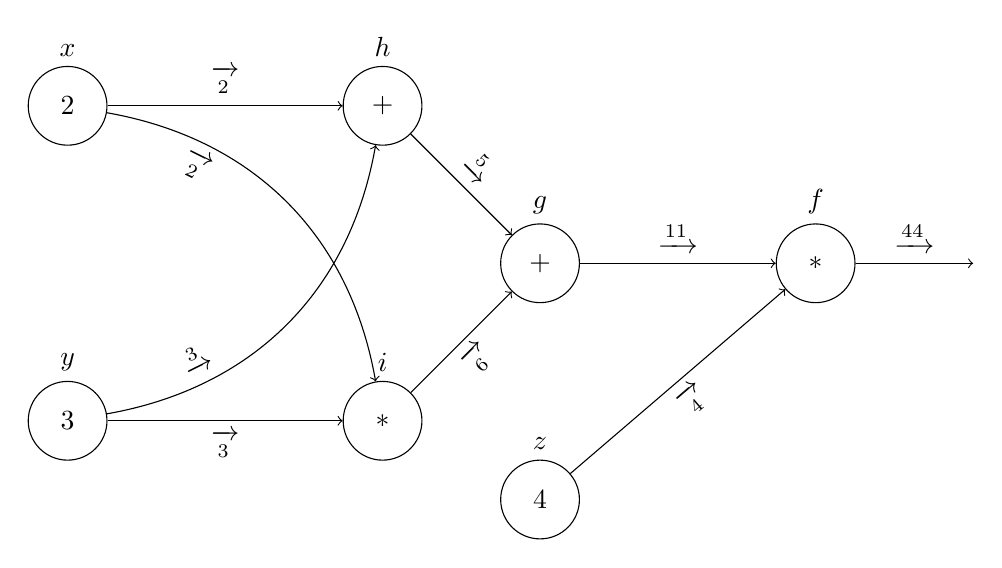
\begin{tikzpicture}
    % nodes: x y h i
    \node[draw, circle, minimum size=1cm, inner sep=0pt, label=$y$] (y) at (0, 0) {$3$};
    \node[draw, circle, minimum size=1cm, inner sep=0pt, label=$i$] (i) at (4, 0) {$*$};
    \node[draw, circle, minimum size=1cm, inner sep=0pt, label=$x$] (x) at (0, 4) {$2$};
    \node[draw, circle, minimum size=1cm, inner sep=0pt, label=$h$] (h) at (4, 4) {$+$};
    % nodes: g z f
    \node[draw, circle, minimum size=1cm, inner sep=0pt, label=$g$] (g) at (6, 2) {$+$};
    \node[draw, circle, minimum size=1cm, inner sep=0pt, label=$z$] (z) at (6, -1) {$4$};
    \node[draw, circle, minimum size=1cm, inner sep=0pt, label=$f$] (f) at (9.5, 2) {$*$};

    % edges: x-h, x-i, y-h, y-i
    \draw[->] (x) to node[sloped, midway, above] {$\xrightarrow[2]{}$} (h);
    \draw[->] (x) to[bend right=-35] node[sloped, near start, below] {$\xrightarrow[2]{}$} (i);
    \draw[->] (y) to[bend right=35] node[sloped, near start, above] {$\xrightarrow[]{3}$} (h);
    \draw[->] (y) to node[sloped, midway, below] {$\xrightarrow[3]{}$} (i);
    % edges: h-g, i-g, g-f, z-f
    \draw[->] (h) to node[sloped, midway, above] {$\xrightarrow[]{5}$} (g);
    \draw[->] (i) to node[sloped, midway, below] {$\xrightarrow[6]{}$} (g);
    \draw[->] (g) to node[sloped, midway, above] {$\xrightarrow[]{11}$} (f);
    \draw[->] (z) to node[sloped, midway, below] {$\xrightarrow[4]{}$} (f);
    % final f edge
    \draw[->] (f) to node[sloped, midway, above] {$\xrightarrow[]{44}$} (11.5, 2);
\end{tikzpicture}

\noindent Now let's formalize this in a more strict methamatical notation:
\begin{enumerate}
    \item $h \;=\; x + y$
    \item $i \;=\; x \times y$
    \item $g \;=\; h + i$, which expands to $g \;=\; (x + y) + (x \times y)$
    \item $f \;=\; g \times z$, which expands to $f \;=\; z \times (x + y) + z \times x \times y$
\end{enumerate}

\noindent This formalization allows us to compute the local gradients as follows:
\begin{enumerate}
    \item For the variable $h$:
        \begin{itemize}
            \item $\frac{\partial h}{\partial x} \;=\; 1,\quad \frac{\partial h}{\partial y} \;=\; 1$
        \end{itemize}

    \item For the variable $i$:
        \begin{itemize}
            \item $\frac{\partial i}{\partial x} \;=\; y \;=\; 3,\quad
                   \frac{\partial i}{\partial y} \;=\; x \;=\; 2$
        \end{itemize}

    \item For the variable $g$:
        \begin{itemize}
            \item $\frac{\partial g}{\partial h} \;=\; 1,\quad \frac{\partial g}{\partial i} \;=\; 1$
        \end{itemize}
    
        \item For the variable $f$:
        \begin{itemize}
            \item $\frac{\partial f}{\partial g} \;=\; z,\quad \frac{\partial f}{\partial z} \;=\; g$
        \end{itemize}
\end{enumerate} \clearpage

\noindent And now we can use the chain rule in order to compute all the derivatives of the graph as
follows (assuming that the derivative of $f$ is 1):
\begin{enumerate}
    \item $f\_\text{to}\_z \,=\, \frac{\partial f}{\partial f} \times \frac{\partial f}{\partial z}
                           \,=\, 1 \times 11 \,=\, 11,\quad
           f\_\text{to}\_g \,=\, \frac{\partial f}{\partial f} \times \frac{\partial f}{\partial g}
                           \,=\, 1 \times 4 \,=\, 4$
    
    \item $f\_\text{to}\_h \,=\, \frac{\partial f}{\partial g} \times \frac{\partial g}{\partial h}
                           \,=\, 4 \times 1 \,=\, 4,\quad
           f\_\text{to}\_i \,=\, \frac{\partial f}{\partial g} \times \frac{\partial g}{\partial i}
                           \,=\, 4 \times 1 \,=\, 4$

    \item $f\_\text{to}\_h\_\text{to}\_x \,=\, \frac{\partial f}{\partial h} \times \frac{\partial h}{\partial x}
                                         \,=\, 4 \times 1 \,=\, 4,\quad
           f\_\text{to}\_i\_\text{to}\_x \,=\, \frac{\partial f}{\partial i} \times \frac{\partial i}{\partial x}
                                         \,=\, 4 \times 3 \,=\, 12$

    \item $f\_\text{to}\_h\_\text{to}\_y \,=\, \frac{\partial f}{\partial h} \times \frac{\partial h}{\partial y}
                                         \,=\, 4 \times 1 \,=\, 4,\quad
           f\_\text{to}\_i\_\text{to}\_y \,=\, \frac{\partial f}{\partial i} \times \frac{\partial i}{\partial y}
                                         \,=\, 4 \times 2 \,=\, 8$
\end{enumerate}
which in turn gives us the complete computational graph:

\bigskip
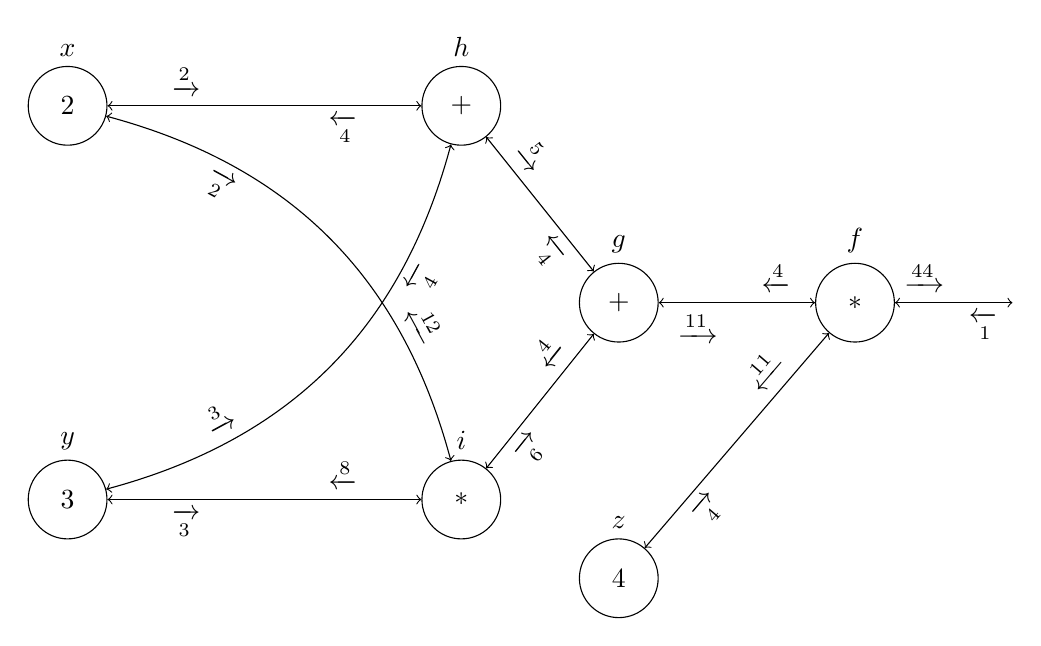
\begin{tikzpicture}
    % nodes: x y h i
    \node[draw, circle, minimum size=1cm, inner sep=0pt, label=$y$] (y) at (0, 0) {$3$};
    \node[draw, circle, minimum size=1cm, inner sep=0pt, label=$i$] (i) at (5, 0) {$*$};
    \node[draw, circle, minimum size=1cm, inner sep=0pt, label=$x$] (x) at (0, 5) {$2$};
    \node[draw, circle, minimum size=1cm, inner sep=0pt, label=$h$] (h) at (5, 5) {$+$};
    % nodes: g z f
    \node[draw, circle, minimum size=1cm, inner sep=0pt, label=$g$] (g) at (7, 2.5) {$+$};
    \node[draw, circle, minimum size=1cm, inner sep=0pt, label=$z$] (z) at (7, -1) {$4$};
    \node[draw, circle, minimum size=1cm, inner sep=0pt, label=$f$] (f) at (10, 2.5) {$*$};

    % edges: x-h, x-i, y-h, y-i
    \draw[<->] (x) to node[sloped, near start, above] {$\xrightarrow[]{2}$}
                      node[sloped, near end, below] {$\xleftarrow[4]{}$} (h);
    \draw[<->] (x) to[bend right=-30] node[sloped, near start, below] {$\xrightarrow[2]{}$}
                                      node[sloped, near end, above] {$\xleftarrow[]{12}$} (i);
    \draw[<->] (y) to[bend right=30] node[sloped, near start, above] {$\xrightarrow[]{3}$}
                                     node[sloped, near end, below] {$\xleftarrow[4]{}$} (h);
    \draw[<->] (y) to node[sloped, near start, below] {$\xrightarrow[3]{}$}
                      node[sloped, near end, above] {$\xleftarrow[]{8}$} (i);
    % edges: h-g, i-g, g-f, z-f
    \draw[<->] (h) to node[sloped, near start, above] {$\xrightarrow[]{5}$}
                      node[sloped, near end, below] {$\xleftarrow[4]{}$} (g);
    \draw[<->] (i) to node[sloped, near start, below] {$\xrightarrow[6]{}$}
                      node[sloped, near end, above] {$\xleftarrow[]{4}$} (g);
    \draw[<->] (g) to node[sloped, near start, below] {$\xrightarrow[]{11}$}
                      node[sloped, near end, above] {$\xleftarrow[]{4}$} (f);
    \draw[<->] (z) to node[sloped, near start, below] {$\xrightarrow[4]{}$} 
                      node[sloped, near end, above] {$\xleftarrow[]{11}$} (f);
    % final f edge
    \draw[<->] (f) to node[sloped, near start, above] {$\xrightarrow[]{44}$}
                      node[sloped, near end, below] {$\xleftarrow[1]{}$} (12, 2.5);
\end{tikzpicture}
\bigskip

Hope you appreciate the above computational graph as it took me a whole day to
learn how the tikz library works :)


\clearpage
% ------------------------------      EXERCISE 5      ----------------------------------- %
\section*{Exercise 5}
I will be thrifty in this report, as most of the explanation is done inside the
Colab Notebook. I have implemented 2 models:
\begin{enumerate}
    \item A Neural Network that uses tfidf to extract features from the Dataset.
    \item A Neural Network that uses the pretrained GloVe embeddings. 
\end{enumerate}

Both models are feedforward Neural Networks. To be honest there is nothing
extremely special about them. Their architectures can be found in the Notebook.
I will go briefly over the different hyperparameters that I hand-tuned, in order
to see what changes took place.

% -----------------------        TFIDF          ------------------------ %
\subsection*{NN with tfidf as input}
\begin{itemize}
    \item \underline{Hyperparameters}
        \smallskip

\begin{enumerate}

    % ----------       HIDDEN LAYERS        ------------ %
    \item \underline{Number of Hidden Layers}
        \smallskip

        Adding up to 3 Hidden Layers improved the models performance. After the
        third layer not much was changing. The Validation Loss and the Validation
        F1-score remained steady.

    % ---------------      NEURONS       ----------------%
    \item \underline{Neurons in Fully Connected Layers}
        \smallskip

        Increasing the number of neurons, in this case, did not affect a lot the performance
        of the model. Instead it slowed down training (especially if many neurons were placed
        in the first hidden layer). Decreasing on the other hand (up until 64-32 in the 1st and
        2nd layers) let to decrease in performance, but faster training.
    % ---------------      ACTIVATIONS       ----------------%
    \item \underline{Activation Functions}
        \smallskip

        Let's start by stating that every model in the end uses a sigmoid activation
        function as we have a binary classification problem. After that, between the
        Linear Layers, the following activations were tried:
        \begin{itemize}
            \item ReLU
            \item SeLU
            \item LeakyReLU ($\alpha=15$)
        \end{itemize}
        To be honest not much difference was shown when changing activation functions.
        I also tried combining these functions (e.g. 1 layer with ReLU and the next with
        SeLU and vice versa). Small improvements were shown when using SeLU.
    % ----------------    DROPOUT    ------------------ %
    \item \underline{Dropout}
        \smallskip

        As expected, adding dropout (with probability $p = 0.15$) helped in generalization
        as it increased validation F1-score by 0.02.

    % ----------------    BATCH NORMALIZATION    ------------------ %
    \item \underline{Batch Normalization}
        \smallskip

        Batch Normalization increased a bit the performance of the model, specifically it
        helped in decreasing the loss down by 0.02.

    % ---------------      LOSS       ----------------%
    \item \underline{Loss Function}
        \smallskip

        Since we are dealing with a Binary Classification problem, I used the Binary
        Crossentropy loss. It words good. I didn't experiment further with this, as I
        did not have much time.

    % ---------------      OPTIMIZER       ----------------%
    \item \underline{Optimizer}
        \smallskip

        SGD, Adam and RMSprop were tried. Adam outperformed all of them, but it slowed down
        the training time a bit. I used RMSprop in the end just for the sake of difference with
        the second model.

    % -----------------      LEARNING RATE        ---------------- %
    \item \underline{Learning Rate}
        \smallskip

        Optimal value for learning rate was found around $5\times10^{-4}$. Values higher than that
        usually led to divergence, and values lower than that led to slow learning.

    % ----------------        WEIGHT DECAY       ---------------- %
    \item \underline{Weight Decay}
        \smallskip

        Optimal value for the weight decay (ridge regularization penalty, L2) was found around
        $10^{-4}$. Higher values made the model underfit, and lower values let to gradual
        overfitting.
    
    % ------------------       BATCH SIZE       --------------------- %
    \item \underline{Batch Size}
        \smallskip

        It's hard to define an optimal value for the batch size, but by the looks of it,
        32 (as Yann LeCun suggests) works out very well, though it makes training a bit slow.
        Also, since we are using batch normalization, having large batches introduces bias to
        the learning procedure, as the weights learn to rely on the normalization that
        takes place during training. So using a small batch size, in our case, actually
        helps the model generalize.
\end{enumerate}

    \item \underline{Comparison with model from Assignment 1}
        \smallskip

        The model from Assignment 1 seems to be performing better than this one (it had
        0.80 F1-score), but it was trained in the whole Dataset, rather than 1/3 which
        is the case here. The Logistic Regression model is a basically a shallow Neural
        Network, so that's why is performs ok. This model could not perform as good as the
        logistic Regressor, because the logistic regressor could make use of sparse
        matrices in order to speed up training and do more epochs. Still, both models
        seem to be performing nicely, but this problem can better be faced with RNNs,
        and there we will get the highest score.

\end{itemize}



% -----------------------        GLOVE          ------------------------ %
\subsection*{NN with pretrained GloVe Embeddings}
\begin{itemize}
    \item \underline{Hyperparameters}
        \bigskip

\begin{enumerate}

    % ----------       HIDDEN LAYERS        ------------ %
    \item \underline{Number of Hidden Layers}
        \smallskip

        Again, adding up to 2 Hidden Layers improved the models performance. After the
        third layer, the model started to overfit a lot.

    % ---------------      NEURONS       ----------------%
    \item \underline{Neurons in Fully Connected Layers}
        \smallskip

        Increasing the number of neurons, in general, helped improve the performance
        of the model. But after 512 neurons for the first layer, then training became
        way too slow.

    % ---------------      ACTIVATIONS       ----------------%
    \item \underline{Activation Functions}
        \smallskip

        Pretty much the same as with the first model. Sigmoid for the last layer and in between
        the following activations were tested:
        \begin{itemize}
            \item ReLU
            \item SeLU
            \item LeakyReLU ($\alpha=15$)
        \end{itemize}
        Again, pretty much the same results were shown.

    % ----------------    DROPOUT    ------------------ %
        \item \underline{Dropout}
        \smallskip

        As expected, again, adding dropout (with probability $p = 0.3$) helped in
        generalizing, as it increased validation F1-score by 0.01.

    % ----------------    BATCH NORMALIZATION    ------------------ %
    \item \underline{Batch Normalization}
        \smallskip

        Batch Normalization increased a bit the performance of the model, specifically it
        helped in decreasing the loss again by 0.02.

    % ---------------      LOSS       ----------------%
    \item \underline{Loss Function}
        \smallskip

        Again, Binary Crossentropy Loss was used for this Network. Next assignment I will
        experiment with Huber Loss, promise.

    % ---------------      OPTIMIZER       ----------------%
    \item \underline{Optimizer}
        \smallskip

        Adam and RMSprop were tried. Adam outperformed RMSprop, but it was so slow
        (especially in the grid search), so I ended up using RMSprop again.

    % -----------------      LEARNING RATE        ---------------- %
    \item \underline{Learning Rate}
        \smallskip

        Optimal value for learning rate was found around $10^{-4}$. Values much higher than
        that usually led to divergence, and values lower than that led to convergence in local
        minima.

    % ----------------        WEIGHT DECAY       ---------------- %
    \item \underline{Weight Decay}
        \smallskip

        Optimal value for the weight decay (ridge regularization penalty, L2) was found around
        $10^{-3}$. Higher values made the model underfit, and lower values let to gradual
        overfitting.
    
    % ------------------       BATCH SIZE       --------------------- %
    \item \underline{Batch Size}
        \smallskip

        For this Network, again a batch size of $32$ was used. In the beggining I was using $512$,
        but it was too unstable (the metrics would change drastically between each fold), so I
        switched back to 32.

\end{enumerate}

    \item \underline{Comparison with model from Assignment 1}
        \smallskip

        Again, the logistic regressor from Assignment 1 performs better. This is expected,
        as the model in this assignment is very simple: take the word embeddings and
        concatenate them, then add fully connected layers. The model will not be able
        to interpret semantical relations, and the order of words which can make an
        impact in the sentiment. Of course, maybe a better implementation that mine
        could give WAY better results, but as suggested in Piazza, I didn't spend much
        time hand-tuning and searching for optimal hyperprameters to get the best possible
        performance.
\end{itemize}

\clearpage
\subsection*{ROC Curves}
The ROC curves for both models can be seen in graph below (also inside the Notebook):
\smallskip

\hspace*{-0.5cm}
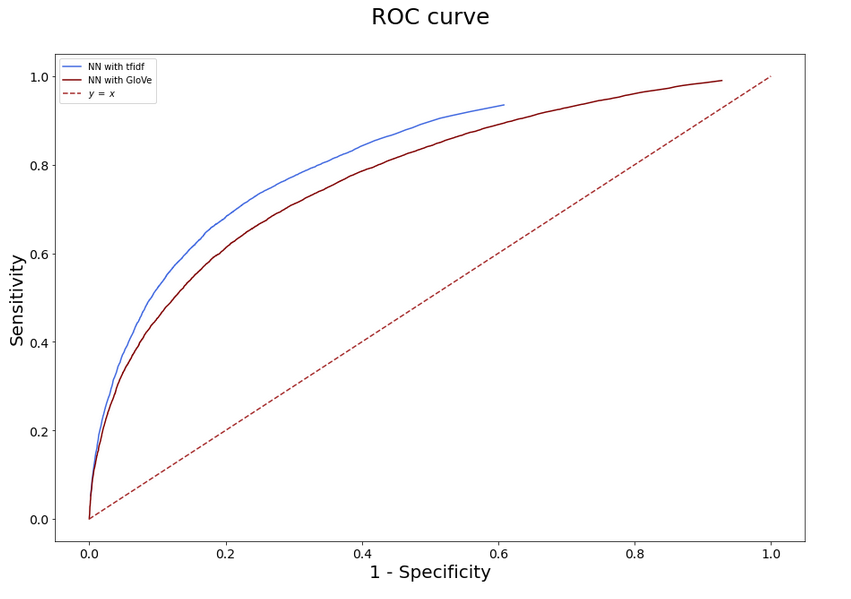
\includegraphics[scale=0.46]{images/roc.png}
\smallskip

It's true that both curves should be intersecting $y\,=\,x$ at $x=1$. They don't because
the thresholds tried were from 0 up to 0.9999 with threshold step size of $0.0001$. In
order for them to touch the $y\,=\,x$ line, we would need to use a smaller threshold step.
Still, this gives us the big picture of how both models perform. The area under a curve,
is a metric of the performance of a model, and it is clear that the first model is
performing better as it has a bigger area.

\subsection*{Best Model}
Without doubt, but unexpectidely, the first model (NN with tfidf) performs better than
the second one which uses GloVe word embeddings. The reasons for this were mostly explained
above in the analysis of each model. But how can we conclude that the first model performs
better? We have the following metrics, measured in the same test set:
\begin{enumerate}
    \item The Loss of the first model is smaller than the loss of the second.
    \item Accuracy of the first model is better than the accuracy of the second.
    \item F1 score of the first model is better than the F1 score of the second.
    \item The are under the ROC curve of the first model is bigger than that of
        the second.
\end{enumerate}
There 4 metrics point us to the fact that the first model performs better.


\end{document}
% ----------------    END OF DOCUMENT    ------------ %
